\documentclass{article}
\usepackage[utf8]{inputenc}
\usepackage{amsmath}
\usepackage{amssymb}
\usepackage{graphicx}

\begin{document}

\section*{Partitioned Matrix}
In this exercise we consider the matrix $\mathbf{A} \in \mathbb{R}^{n+1,n+1}$ composed of four blocks.
\begin{equation*}
    \mathbf{A} = 
    \begin{bmatrix}
    \mathbf{R} & \mathbf{v} \\
    \mathbf{u}^{\mathsf{T}} & 0
    \end{bmatrix}
\end{equation*}
where $\mathbf{v}\in \mathbb{R}^{n}$, $\mathbf{u}\in \mathbb{R}^{n}$ and $\mathbf{R} \in \mathbb{R}^{n \times n}$ is \textbf{upper triangular} and \textbf{regular}.
\subsection*{2-9.a} 
We are tasked with finding a necessary and sufficient condition for the \textbf{triangular} matrix $\mathbf{R}$ to be invertible. Here we remember that the determinant of a triangular matrix $\mathbf{R}$ is given by the product of its diagonal elements. Hence in the case of $\mathbf{R}$ we have
\begin{equation*}
    \text{det}\:\mathbf{R} = \prod_{i=1}^{n}r_{ii}
\end{equation*}
Which means that we have
\begin{equation*}
    \text{det}\:\mathbf{R} \neq 0 \Longleftrightarrow  \prod_{i=1}^{n}r_{ii} \neq 0 \Longleftrightarrow r_{ii} \neq 0 \quad \forall \, 1 \leq i \leq n
\end{equation*}
If  and only if the determinant of $\mathbf{R}$ is non-zero, then the matrix is invertible.
\begin{equation*}
    \mathbf{R} \text{ is invertible } \Longleftrightarrow r_{ii} \neq 0 \quad \forall \, 1 \leq i \leq n
\end{equation*}
\subsection*{2-9.b}
We are now tasked with solving the following block LSE
\begin{equation*}
    \begin{bmatrix}
        \mathbf{R} & \mathbf{v} \\
        \mathbf{u}^{\mathsf{T}} & 0
    \end{bmatrix}
    \begin{bmatrix}
        \mathbf{z} \\
        \chi
    \end{bmatrix}
    = \begin{bmatrix}
        \mathbf{b}\\
        \beta
    \end{bmatrix}
\end{equation*}
for arbitrary $\mathbf{b}\in \mathbb{R}^{n}$ and $\beta \in \mathbb{R}$. We apply the techniques discussed in the section 2.6.0.2 of the lecture document to form an equivalent block partitioned LSE
\begin{align*}
    \mathbf{R}\mathbf{z} + \mathbf{v}\chi &= \mathbf{b} \\
    \mathbf{u}^{\mathsf{T}}\mathbf{z} + 0 \cdot \chi &= \beta
\end{align*}
We must have that $\mathbf{R}$ is regular (invertible) which is given by the exercise. We can directly apply block arithmetic to give us
\begin{align*}
    \mathbf{R}\mathbf{z}  &= \mathbf{b} - \mathbf{v}\chi\\
    \mathbf{u}^{\mathsf{T}}\mathbf{z} &= \beta
\end{align*}
and from this we get
\begin{align*}
    \mathbf{z}  &= \mathbf{R}^{-1}\left(\mathbf{b} - \mathbf{v}\chi\right)\\
    \mathbf{u}^{\mathsf{T}}\mathbf{z} &= \beta
\end{align*}

\pagebreak

\noindent We then use the first equation in the second equation to give us
\begin{equation*}    \mathbf{u}^{\mathsf{T}}\mathbf{R}^{-1}\left(\mathbf{b} - \mathbf{v}\chi\right) = \beta
\end{equation*}
we then have 
\begin{align*}    \mathbf{u}^{\mathsf{T}}\mathbf{R}^{-1}\mathbf{b} - \mathbf{u}^{\mathsf{T}}\mathbf{R}^{-1}\mathbf{v}\chi= \beta &\implies  \left(- \mathbf{u}^{\mathsf{T}}\mathbf{R}^{-1}\mathbf{v}\right)\chi= \beta - \mathbf{u}^{\mathsf{T}}\mathbf{R}^{-1}\mathbf{b} \\
&\implies \chi =  \frac{\beta - \mathbf{u}^{\mathsf{T}}\mathbf{R}^{-1}\mathbf{b}}{- \mathbf{u}^{\mathsf{T}}\mathbf{R}^{-1}\mathbf{v}}
\end{align*}
It is important that $- \mathbf{u}^{\mathsf{T}}\mathbf{R}^{-1}\mathbf{v} \in \mathbb{R}$ and we can hence divide by it, this would otherwise not be possible, we also have to make sure that $\mathbf{u}^{\mathsf{T}}\mathbf{R}^{-1}\mathbf{v}  \neq 0$ as otherwise we cannot divide by it. Hence we get our solutions by solving the following equations in the order stated.
\begin{align*}
    \chi &=  \frac{\beta - \mathbf{u}^{\mathsf{T}}\mathbf{R}^{-1}\mathbf{b}}{- \mathbf{u}^{\mathsf{T}}\mathbf{R}^{-1}\mathbf{v}} \\[1mm]
    \mathbf{z}  &= \mathbf{R}^{-1}\left(\mathbf{b} - \mathbf{v}\chi\right)
\end{align*}
\subsection*{2-9.c}
We can use the fact that a matrix $\mathbf{A}$ is regular if and only if $\mathbf{A}\mathbf{x} = \mathbf{b}$ has a unique solution for any right side $\mathbf{b}$. We see that if $\mathbf{u}^{\mathsf{T}}\mathbf{R}^{-1}\mathbf{v}  \neq 0$ then such a solution exists and is uniquely defined by the two above equations. We can also see that for $\mathbf{u}^{\mathsf{T}}\mathbf{R}^{-1}\mathbf{v} = 0$ the above system has no solution and thus the system itself has no solution, meaning that a right side exists for which the system has no solution, which means that $\mathbf{A}$ would not be regular. \\[2mm]


\noindent An alternative proof which I find very elegant is stating the block LU decomposition, which is given by
\begin{equation*}
    \mathbf{A} = \begin{bmatrix}
        \mathbf{R} & \mathbf{v} \\
        \mathbf{u}^{\mathsf{T}} & 0
    \end{bmatrix}
    = 
    \begin{bmatrix}
        \mathbf{I} & \mathbf{O} \\
        \mathbf{u}^{\mathsf{T}} & \mathbf{I}
    \end{bmatrix}
    \begin{bmatrix}
        \mathbf{R} & \mathbf{v} \\
        \mathbf{O} & -\mathbf{u}^{\mathsf{T}}\mathbf{R}^{-1}\mathbf{v}
    \end{bmatrix}
\end{equation*}
We can see that if $\mathbf{u}^{\mathsf{T}}\mathbf{R}^{-1}\mathbf{v} = 0$, then the bottom row of the $\mathbf{U}$ matrix vanishes, making it non-regular, because $\mathbf{L}$ is triangular and has the determinant $1$ (all diagonal elements are $1$), we determine regularity of $\mathbf{A}$ only based on the regularity of $\mathbf{U}$, which depends on if $\mathbf{u}^{\mathsf{T}}\mathbf{R}^{-1}\mathbf{v} = 0$ or not.
\subsection*{2-9.d}
We now tasked with implementing a function that efficiently solves the system $\mathbf{A}\mathbf{x} = \mathbf{b}$ for the described matrix $\mathbf{A}$ and the vector $\mathbf{b}$. We should also implement size checks. We are given the hint that we are allowed to rely on the \verb|triangularView()| function to inform Eigen on the triangular structure of $\mathbf{R}$. 

\pagebreak

\noindent What is meant by the the hint is that we can use $\\[2mm]$
\verb|Eigen::TriangularView<Eigen::MatrixXd, Eigen::Upper>| $\\$

\noindent and the \verb|solve()| utility that comes with it. Let us look at the system we plan on solving.

\begin{align*}
    \chi &=  \frac{\beta - \mathbf{u}^{\mathsf{T}}\mathbf{R}^{-1}\mathbf{b}}{- \mathbf{u}^{\mathsf{T}}\mathbf{R}^{-1}\mathbf{v}} \\[1mm]
    \mathbf{z}  &= \mathbf{R}^{-1}\left(\mathbf{b} - \mathbf{v}\chi\right)
\end{align*}
Here we have three places where we could use a \verb|solve()| call first to find $\mathbf{R}^{-1}\mathbf{b}$, for $\mathbf{R}^{-1}\mathbf{v}$  and then to find the solution of $\mathbf{z}$. Again we find this by solving the system below for some placeholder variable $\mathbf{x}$
\begin{align*}
    \mathbf{R}\mathbf{x} = \mathbf{v} &\implies \mathbf{x} = \mathbf{R}^{-1}\mathbf{v} \\
    \mathbf{R}\mathbf{x} = \mathbf{b} &\implies \mathbf{x} = \mathbf{R}^{-1}\mathbf{b} \\
    \mathbf{R}\mathbf{z} = \mathbf{b} - \mathbf{v}\chi &\implies \mathbf{z} = \mathbf{R}^{-1}\left(\mathbf{b} - \mathbf{v}\chi\right)
\end{align*}

\begin{figure}[!hbt]
    \centering
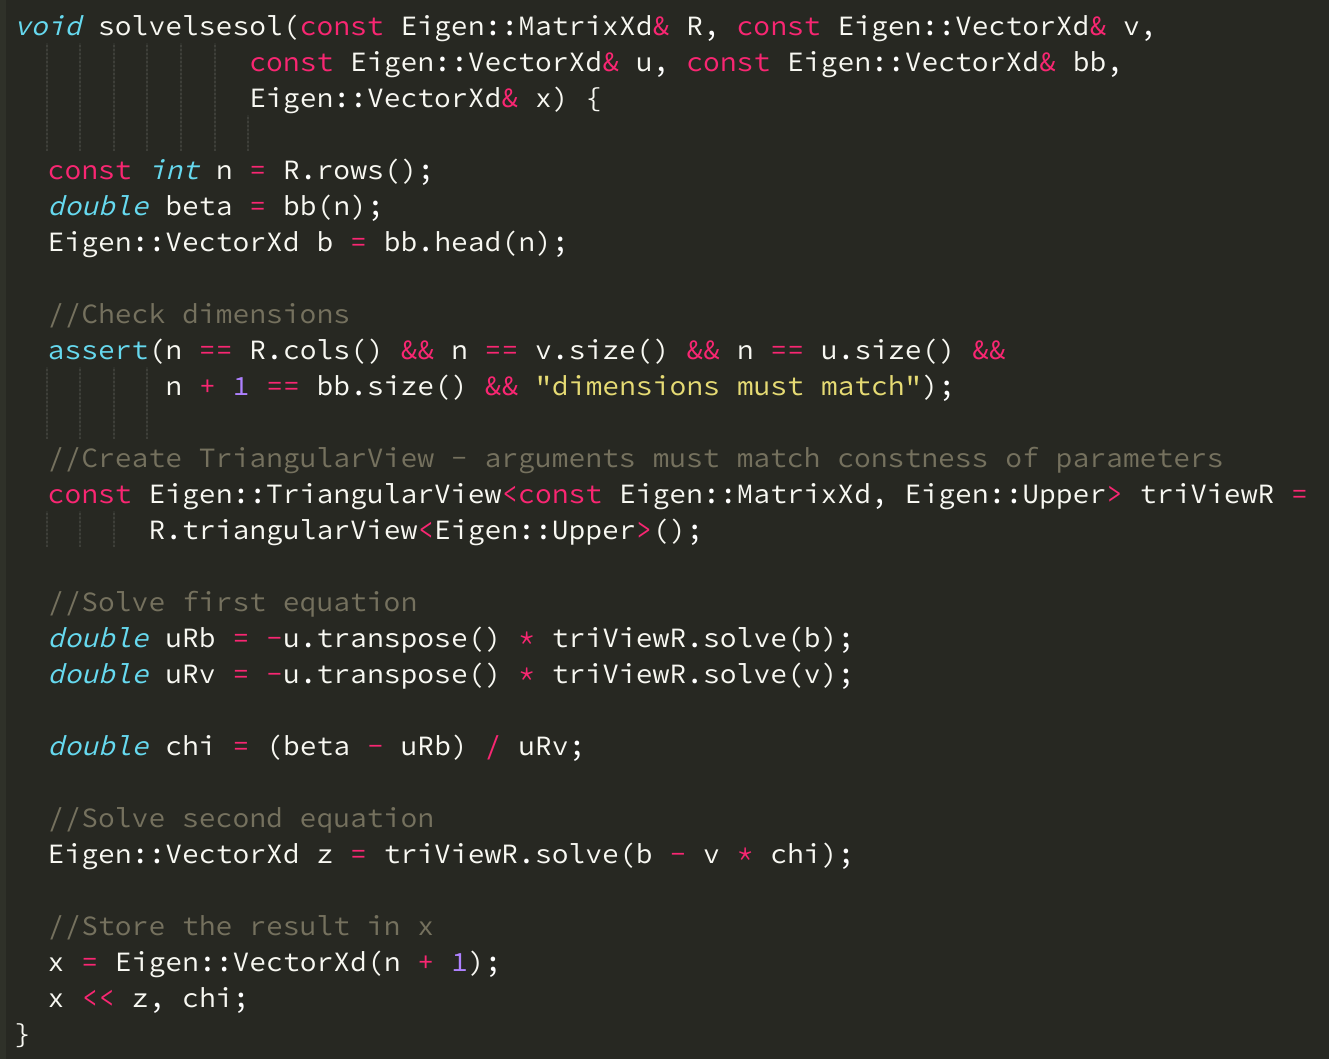
\includegraphics[width=1.0\linewidth]{2-9.d.png}
\end{figure}

\pagebreak

\subsection*{2-9.e}
We are tasked with writing a test function that returns true if the LU based solver returns the same result as the method implemented before. The main difficulty here is to recongnize that we cannot just check for equality because of numerical instability, hence we will use the following norm based comparison instead for result vectors $\mathbf{v}, \mathbf{u}$
\begin{equation*}
    \left\lVert \mathbf{u} - \mathbf{v}\right\rVert_{2} < \text{tol} \cdot \left\lVert \mathbf{b}\right\rVert_{2}
\end{equation*}
We will choose \verb|1e-8| here, because machine precision is not reasonable as multiple errors could stack up. This results in the following code.

\begin{figure}[!hbt]
    \centering
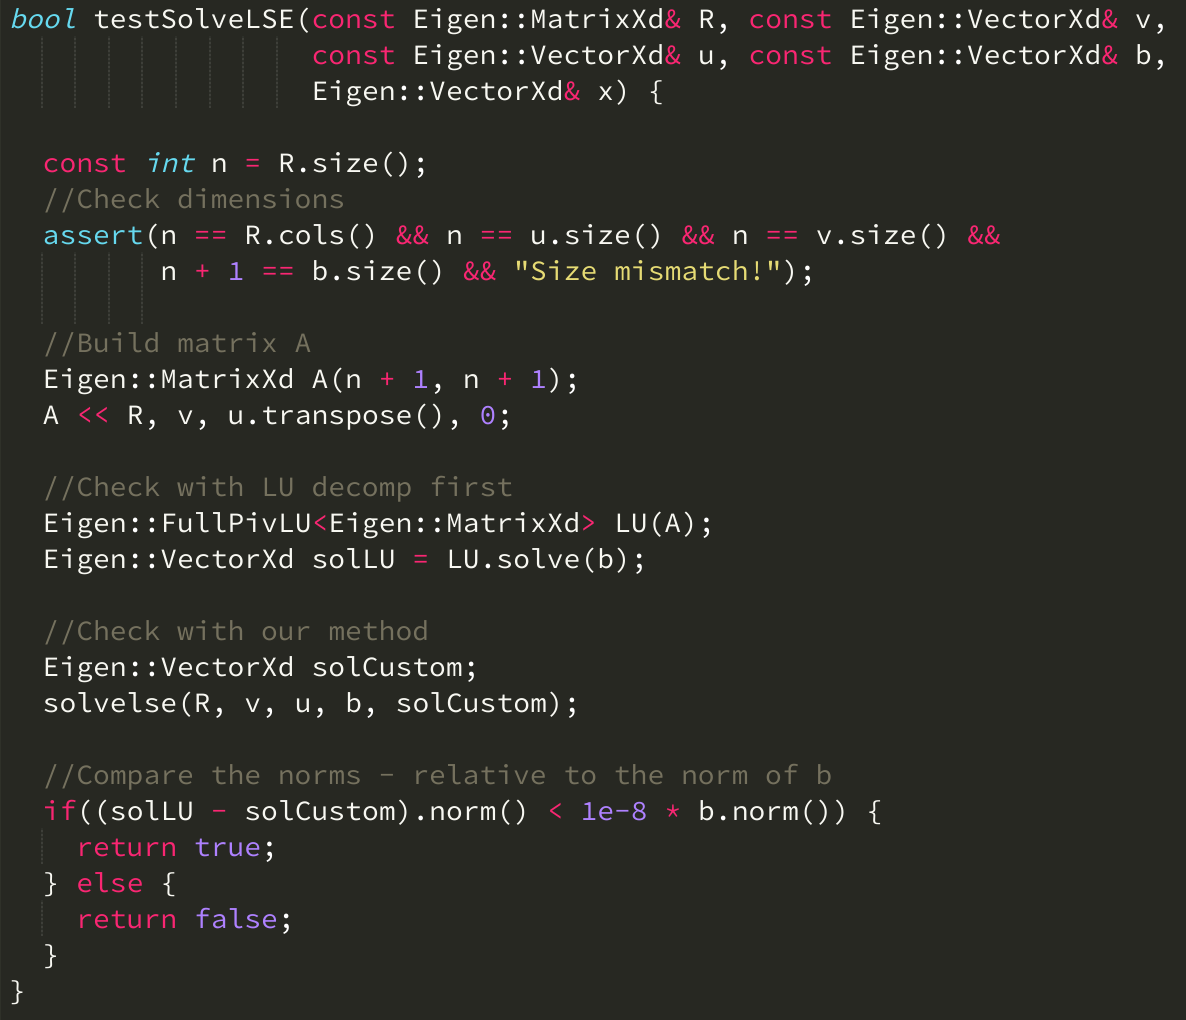
\includegraphics[width=1.0\linewidth]{2-9.e.png}
\end{figure}

\noindent Remember that \verb|FullPivLU| resides in \verb|<Eigen/LU>| and that we must consider the norm of $\mathbf{b}$, because the relative error must scale with the norm of the solution, as a small error might be large in comparison to the vector norm of $\mathbf{b}$, but the vector norm of $\mathbf{b}$ might also be large and thus the error is negligible in that case.
\subsection*{2-9.f} 
We are now tasked with determining the asymptotic complexity of the code implemented in $2-9.d$. Solving and constructing a triangular system takes $\mathcal{O}\left(n^{2}\right)$, as we solve such a system three times we get $\mathcal{O}\left(n^{2}\right)$. The inner products we also compute before we use the solver can be done in $\mathcal{O}\left(n\right)$, hence overall we get $\mathcal{O}\left(n^{2}\right)$.


\end{document}
